%%%%%%%%%%%%%%%%%%%%%%% file template.tex %%%%%%%%%%%%%%%%%%%%%%%%%
%
% This is a general template file for the LaTeX package SVJour3
% for Springer journals.          Springer Heidelberg 2010/09/16
%
% Copy it to a new file with a new name and use it as the basis
% for your article. Delete % signs as needed.
%
% This template includes a few options for different layouts and
% content for various journals. Please consult a previous issue of
% your journal as needed.
%
%%%%%%%%%%%%%%%%%%%%%%%%%%%%%%%%%%%%%%%%%%%%%%%%%%%%%%%%%%%%%%%%%%%
%
% First comes an example EPS file -- just ignore it and
% proceed on the \documentclass line
% your LaTeX will extract the file if required

%
\RequirePackage{fix-cm}
%
%\documentclass{svjour3}                     % onecolumn (standard format)
%\documentclass[smallcondensed]{svjour3}     % onecolumn (ditto)
\documentclass[twocolumn]{svjour3}       % onecolumn (second format)
%\documentclass[twocolumn]{svjour3}          % twocolumn
%
\smartqed  % flush right qed marks, e.g. at end of proof
%
\usepackage{graphicx}
%
% \usepackage{mathptmx}      % use Times fonts if available on your TeX system
%
% insert here the call for the packages your document requires
%\usepackage{latexsym}
% etc.
%
% please place your own definitions here and don't use \def but
% \newcommand{}{}
%
% Insert the name of "your journal" with
% \journalname{myjournal}
%
\begin{document}

\title{Confocal Raman Thermometer for Microfluidic Devices}
%\thanks{Grants or other notes
%about the article that should go on the front page should be
%placed here. General acknowledgments should be placed at the end of the article.

%\subtitle{Do you have a subtitle?\\ If so, write it here}

%\titlerunning{Short form of title}        % if too long for running head

\author{Guillermo D. Brinatti Vazquez         \and
        Oscar E. Mart\'{i}nez \and
        Juan Mart\'{i}n Cabaleiro %etc.
}

%\authorrunning{Short form of author list} % if too long for running head

\institute{F. Author \at
              first address \\
              Tel.: +123-45-678910\\
              Fax: +123-45-678910\\
              \email{fauthor@example.com}           %  \\
%             \emph{Present address:} of F. Author  %  if needed
           \and
           S. Author \at
              second address
}

\date{Received: date / Accepted: date}
% The correct dates will be entered by the editor


\maketitle

\begin{abstract}
\keywords{First keyword \and Second keyword \and More}
\end{abstract}

\section{Introduction}

\section{Experimental}

The setup used to measure the temperature in the microchannels is depicted in figure \ref{fig:setup}. The device works as a confocal microscope, where the traditional pinhole is replaced with a multimode optical fiber. The excitation beam is a 50 mW single mode fiber couple laser diode emitting at a wavelength of 405 nm. Beam is collimated by a lens (CL1) and a short pass filter with 450 nm cutoff wavelength (450 SP) is used to eliminate any noise at the signal beam wavelength (around 470 nm).
%The beam is spatially filtered using a single mode optical fiber to achieve a nearly gaussian spatial mode before entering the microscope. To achieve a tighter focus at the sample plane a 3.6X telescope is used to increase beam waist after the spatial filter. 
At this point, a longpass dichroic mirror (420 LP) splitting in 420 nm is used to reflect the excitation beam in the direction of the sample. The beam then reflects in a second dichroic mirror (505 LP) centered around 505 nm and then is focused on the sample using a 40X, 0.95 NA microscope objective (OL). The final optical power at the sample is 25 mW at 405 nm. The backscattered Raman emission of the sample is collected by the same microscope objective and directed to the optical fiber. As the Raman spectrum of water is centered around 470 nm, the signal beam will reflect in the first dichroic mirror (505 LP) and then transmit on the second (420 LP). After that, the light is directed to the multimode optical fiber by using two mirrors. A 10X, 0.28 NA microscope objective (FL) is used to focus the beam in the optical fiber which is mounted in a 3 axis micrometric linear translation stage. This allows a confocal collection volume of 40 $\mathrm{\mu m^3}$ with an axial resolution of 9 $\mathrm{\mu m}$. The sample is mounted in a platform with tree motorized linear degrees of freedom (\textit{xyz}) and two manually controlled angular (\textit{pitch} and \textit{yaw}) degrees of freedom used to place the sample parallel to the detection plane. This allows the device to make three dimensional temperature maps of the sample. A galvo mirror scanning scheme is also possible to achieve faster or higher spatial resolution imaging.

\begin{figure}[h!]\label{fig:setup}
\centering
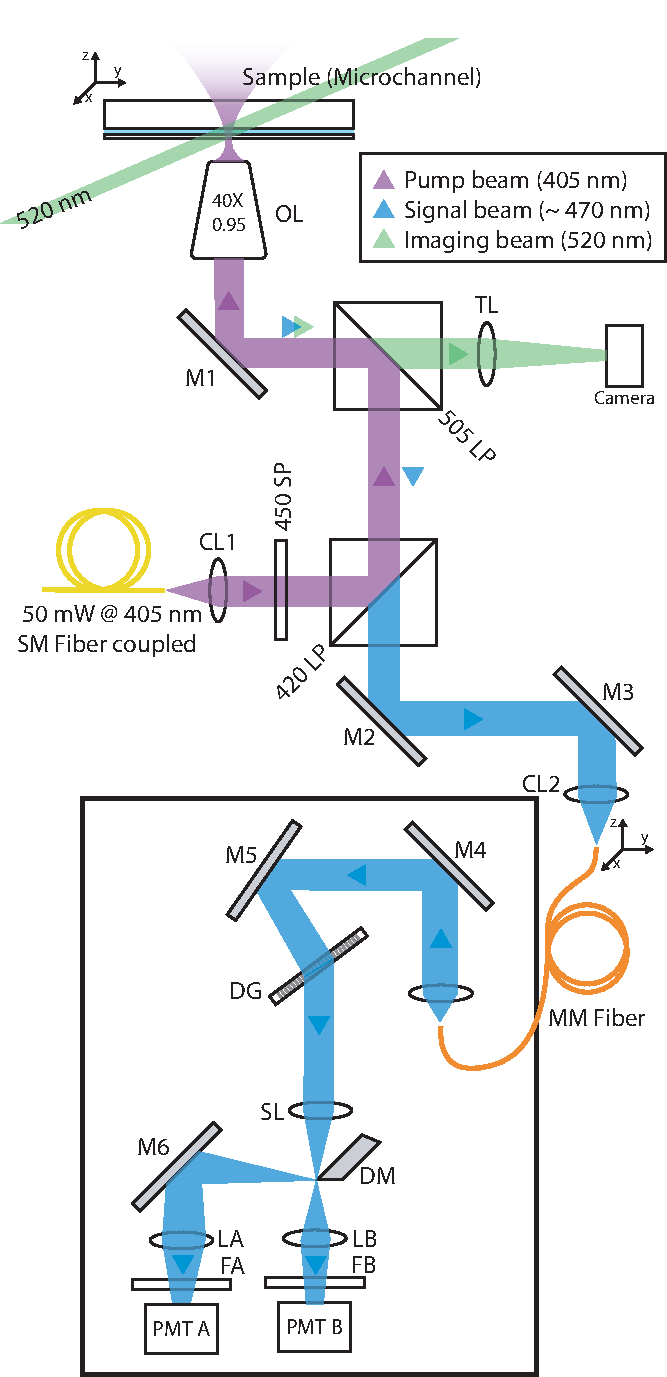
\includegraphics[width=\columnwidth]{figs/setup.eps}
\caption{Schematic representation of the confocal microscope used for Raman thermometry of water. A 405 nm single mode fiber coupled laser is used as excitation beam. The beam is focused in the sample by using a 40X microscope objective who also collects the Raman emission. A dichroic mirror (420 LP) is used to separate the signal which is then focused on a multimode optical fiber to achieve confocal resolution. The other end of the fiber enters a specially designed spectrometer which divide the Raman spectrum in two detectors for later processing. A different wavelength (520 nm) is used to get a scattering image of the sample which is separated from the signal and the pump beam by means of a dichroic mirror (505 LP) and sent to a CCD camera. Colored arrows indicate the wavelength and the propagation direction of each beam.}
\end{figure}

 At the same time Raman measurements are being performed a longer wavelength can be used to get a fluorescence or scattering image of the sample. With this purpose a 10 mW laser beam at 520 nm is used to illuminate the sample in an angle greater than the collection angle of the objective (71.8 $\deg$ for a 0.95 NA objective). The scattered light or the emitted fluorescence is then collected and separated from the Raman beam using the first dichroic mirror (520 LP) which is transparent at these wavelengths. Then, a 100 mm tube lens (TL) is used to get an image of the sample plane at a CMOS camera (Pixelink PL-D725). Using this method an image of the sample can be achieved without interfering with the Raman measurements. This can be used to select a particular place in the sample to perform the temperature measurements or to monitor the fluid motion if fluorescent particles are added to the studied fluid. In the latter case a longpass optical filter should be placed before the camera to eliminate any scattering component at the laser wavelength. If this method is performed, care must be taken in the type and concentration of the particles used, as an undesired fluorescence signal might be excited by the 405 nm beam and collected in the Raman channel if it passes through the confocal volume. But, as the latter is designed to be small, at low particle concentrations the probability of such event can be small enough to not interfere with the temperature measurements. Also, as the Raman cross section of water is low, the contribution to the total signal in the Raman channel of a fluorescent particle passing rapidly through the confocal volume is a sharp peak which can be easily filtered of the temperature signal which is generally expected to be smooth. 
 
At the other end of the multimode optical fiber the Raman signal beam is divided in the two spectral bands necessary for the temperature measurement and then detected. For this purpose a transmission diffraction grating (DG) with 300 l/mm and a 200 mm achromatic lens (SL) is used as a simple spectrometer. A D shaped mirror (DM) is used in the lens focal plane to separate the two spectral bands. The latter is mounted in a micrometric translation stage which allows a fine tunning of the separation wavelength which must be matched to the isosbectic point in order to maximize the temperature sensitivity of the method. After this both reflected and transmited beam are directed to the detectors. A 75 mm lens (LA and LB) is used in each path to make a one on one image of DM in each detector. A longpass filter centered at 450 nm (FA and FB) is used in each channel to reject the laser wavelength. The detectors are two photon counting modules (Hamamatsu H7828) providing a quantum efficiency of around 15\% at the desired wavelength. The devices are designed to produce an amplified and shaped square pulse for each detected photon simplifying the photon counting procedure. The pulses are then counted in a selectable time window using an on board DAQ device on a PC. Counting rates of around $1.5 \cdot 10^5 \,\,\mathrm{s}^{-1}$ are achieved at each channel. After this, the final signal is computed at software level as
\begin{equation}\label{eq:S}
S = \frac{B – A}{A + B}
\end{equation}
where A and B are the counts of each channel. The temperature of the sample is obtained from this calculation after proper calibration.  It is important to notice that $S$ is computed as a ratio, making the calibration independent of experimental parameters such as the excitation power or the integration time.

Additionally the diffraction grating (DG) is mounted in a motorized rotation stage.  This is not completely necessary to the Raman measurements but allows using the device as a spectrometer by measuring the signal as a function of the incidence angle on the grating and then taking the numeric derivative of the data. This simplifies the procedure of choosing the isosbectic point and allows checking the detected spectrum to match the one of water, confirming the proper alignment of the microscope. 

As the detectors are very sensitive and the Raman signal is very low, the whole detection part of the setup is enclosed in an opaque box to avoid ambient light reaching the detectors. This is a great advantage of using an optical fiber to produce the confocal resolution instead of a pinhole as the ambient light coupled to the fiber is practically null and the signal beam can be conveniently directed to the enclosed part of the setup, allowing a much relaxed illumination constrain in the laboratory. 

To calibrate the method a temperature controlled water cell was used. This was constructed using a rectangular aluminum plate with a perforation sealed with two glass windows and containing around 150 $\mu$l of distilled water. A peltier cell was fixed at one side of the piece to achieve either heating or cooling and a thermistor is used to monitor the piece temperature.  Placing this cell in the sample plane of the microscope allows a temperature controlled water sample used to set the isosbestic point and to calibrate the method. 

Aca iria un parrafo contando las caracteristicas de los microcanales que usamos como muestra (tal vez convenga pedirle a Martin que lo escriba o que nos diga que es relevante decir sobre el proceso con el que los armo). Cosas que pienso que van: que están pegados a cubres de 150 um. Que se uso KCl para setear la conductividad en 5000 mS/cm. Las medidas de los canales. Que se alimento con una fuente de tensión regulable de hasta 1kV logrando los campos eléctricos …



\section{Results and Discussion}

To characterize the technique a series of Raman spectra were measured at different temperatures. This was performed by using a pure water sample in the temperature controlled cell and by scanning the angle on the diffraction grating. After taking the numeric derivative, the recovered spectra is shown in figure \ref{fig:spectra}. Results show an isosbestic point around 470 nm in agreement with previous measurements\cite{walrafen1}. As temperature increase, the shorter wavelength components of the Raman spectrum reduce their intensity while the longer wavelength part slightly increases. The total spectrum collected in each detector (channel A and B) is shaded in light blue and red. This measurements are used to set the angle at which the spectrum is split exactly at the isosbectic point, leading to the maximum temperature sensibility. 

\begin{figure}[h!]
\centering
\includegraphics[width=\columnwidth]{figs/spectra.eps}
\label{fig:spectra}
\caption{Raman spectra of water at different temperatures. A dashed line marks the isosbestic point. At shorter wavelengths the signal decreases with rising temperature. At longer wavelengths the opposite behavior occurs. Shaded regions indicate the portion of the spectrum collected in each detector in the temperature measurements as shown in figure \ref{fig:setup}.}
\end{figure}

Having set the spectrometer properly, a calibration is made by computing the quantity $S$, as defined in equation \ref{eq:S}, as a function of temperature. The result from this experiment is shown in figure \ref{fig:calib} where a linear behavior is exhibited in the range of interest. A linear fit is finally used to obtain the calibration curve. With this calibration and by measuring the noise in the temperature signal  the resolution of the method can be estimated. The result of this experiment is consistent with the spread of the data around the linear fit in figure \ref{fig:calib} with a value of 0.8 K for a integration time of one second.

\begin{figure}[h!]
\centering
\includegraphics[width=\columnwidth]{figs/calib.eps}
\label{fig:calib}
\caption{Temperature signal $S$ as a function of the water sample temperature. A linear fit is used as calibration for the method. Dispersion around the linear fit gives a temperature resolution of $\Delta T = 0.8$ K.}
\end{figure}

With this results a full characterization of the thermal properties of the microchannels under electroosmotic flow is possible. First of all, the the temperature rise at \textit{turn on} is studied, from ambient temperature (when the electric field is turned off) to the equilibrium temperature once the flow is established. The result of this experiment for a channel with dimensions b = 80 $\mathrm{\mu m}$, h = 100 $\mathrm{\mu m}$ and $L$ = 20 mm is shown if figure \ref{fig:temporal}. Electric field is turned on at $t = 0$. The flow velocity was measured to be 1 mm/s. A temperature rise of 12 K is observer in a short time (around 10 seconds) for two different positions in the channel 5 mm apart. This timing is independent of the position of the channel, showing no mass transport effects.

\begin{figure}[h!]
\centering
\includegraphics[width=\columnwidth]{figs/temporal.eps}
\label{fig:temporal}
\caption{Temperature rise at turn on for a microchannel under elecroosmotic flow. Electric field is activated at $t=0$. Two different positions 5 mm apart show the same behavior. The position $x=0$ is set at the inlet reservoir. (Channel dimensions  b = 80 $\mathrm{\mu m}$, h = 100 $\mathrm{\mu m}$ and $L$ = 20 mm)}
\end{figure}

As mentioned before, the advantage of a confocal collection scheme is that spatial temperature maps can be performed. In figure \ref{fig:horizontal} we start by showing a lateral scan (perpendicular to the flow direction, parallel to the coverglass) in a channel of dimensions b = 80 $\mathrm{\mu m}$, h = 100 $\mathrm{\mu m}$ and $L$ = 40 mm and once a stationary temperature was established. Despite some noise, a constant 13 K increase in temperature is observed compared to ambient temperature. The sensing close to the walls of the channel is not possible due to a strong fluorescence signal coming from the PDMS. This limitation might not be the case in other manufacturing materials.

\begin{figure}[h!]
\centering
\includegraphics[width=\columnwidth]{figs/horizontal.eps}
\label{fig:horizontal}
\caption{Horizontal scan (perpendicular to the flow, parallel to the coverglass) showing a constant temperature rise across the channel (Channel dimensions  b = 80 $\mathrm{\mu m}$, h = 100 $\mathrm{\mu m}$ and $L$ = 40 mm).}
\end{figure}

In figure \ref{fig:vertical} a vertical scan is shown for the same chip and for two different total dissipated powers on the water. Here, sensing near the ceiling of the channel is not possible (again due to PDMS fluorescense) but it is near the floor as glass exhibit no fluorescence. Because of this, data points are shown from the center of the channel to the glass surface, where the signal starts decaying as the collection volume starts sensing the glass space (and temperature SNR starts decreasing). Again, similar to what was shown in figure \ref{fig:horizontal}, temperature exhibit a constant behaviour on the whole vertical scan.

\begin{figure}[h!]
\centering
\includegraphics[width=\columnwidth]{figs/vertical.eps}
\label{fig:vertical}
\caption{Two vertical scans at different dissipated powers in the same channel used in figure \ref{fig:horizontal}. Position zero corresponds to the center of the channel. On the right side lays the coverglass.}
\end{figure}

The final spatial scan is shown in figure \ref{fig:long} where a longitudinal scan was performed. Again, temperature shows a constant behavior along the channel, similar to what was shown in figure \ref{fig:temporal}. This is consistent with theoretical calculations \cite{jouleteorico} where temperature rise occurs in the very beginning of the channel and then a constant value is achieved. A simple calculation considering that all heat flows trough the floor of the channel (glass) can be useful to estimate the required temperature gradient needed to reach a stationary regime where the extracted heat compensates Joule effect. For a typical dissipated power of 40 mW and a channel of dimensions $b = h = 100$ $\mathrm{\mu m}$ and $L$ = 20 mm the required temperature difference between the ceiling and the floor is 

\begin{equation}
\Delta T = \frac{Ph}{kLb} = 1.7\,\, \mathrm{K},
\end{equation}

where $P$ is Joule heat dissipated on the channel and $k$ is water thermal conductivity. This upper bound is already on the limits of what is measurable with the technique and then our measurements are consistent with the glass base of the channel dominating as dissipation mechanism. 

\begin{figure}[h!]
\centering
\includegraphics[width=\columnwidth]{figs/long.eps}
\label{fig:long}
\caption{Longitudinal scan across a L = 20 mm channel. The experiment show a constant temperature rise around 13 K. }
\end{figure}

To confirm this hypothesis curves of temperature rise as function of dissipated power per unit glass area were measured for different channel geometries. The result of this experiment is plotted in figure \ref{fig:rectas}. A linear fit was performed for each data set. Results show that all different geometries have a similar slope, proving that glass area is the most relevant parameter defining heat dissipation out of our channels. This is also consistent with results from other groups \cite{competencia1} where rectangular channels made completely out of PDMS exhibit higher temperatures and longitudinal variations with similar conductivity and applied field. 

\begin{figure}[h!]
\centering
\includegraphics[width=\columnwidth]{figs/rectas.eps}
\label{fig:rectas}
\caption{Temperature rise as a function of dissipated power per unit glass area on four different channel geometries. A linear fit is performed in each data set in order to compare the slope corresponding to each channel. The similarity between the lines seems to indicate that the glass floor of the channel dominates as dissipation mechanism.}
\end{figure}

\bibliographystyle{spphys}
\bibliography{bibliography}

% BibTeX users please use one of
%\bibliographystyle{spbasic}      % basic style, author-year citations
%\bibliographystyle{spmpsci}      % mathematics and physical sciences
%\bibliographystyle{spphys}       % APS-like style for physics
%\bibliography{}   % name your BibTeX data base


\end{document}

